\documentclass[a4j]{jarticle}
\usepackage[dvipdfmx]{graphicx}
\usepackage{float}
\usepackage{jcfd39}
\usepackage{amsmath}
\usepackage{url}
\usepackage{placeins}
\usepackage{subcaption}
%
%\usepackage{ulem} %proofreading e.g. \uuline{ \uwave{  \sout{demo}}}
%
%\makeatletter  % Change the style of citation and biblabal - II
%\def\@cite#1{$^{\mbox{\scriptsize{(#1})}}$}
%\makeatother

\newcommand{\ctext}[1]{\raise0.2ex\hbox{\textcircled{\scriptsize{#1}}}}


%%\def\papernum{講演番号}                %講演番号を記して下さい

\title{2次元直交格子を用いたShock-Fitting法の基礎的研究}   %和文タイトルを記して下さい
\etitle{Fundamental Study on the Shock-Fitting Method Using 2D Cartesian grid}   %英文タイトルを記して下さい
                                    %和文著者名を記して下さい
\author{\begin{tabular}{cl}
$\bigcirc$ & 西尾朋人,東大, 
             東京都文京区本郷7-3-1, 
             E-mail:nishio-tomohito048@g.ecc.u-tokyo.ac.jp \\
           & 今村太郎,東大,
             東京都文京区本郷7-3-1, 
             E-mail:imamura@g.ecc.u-tokyo.ac.jp
\end{tabular} }

                                    %英文著者名を記して下さい
\eauthor{\begin{tabular}{l}
    Tomohito NISHIO, 
    The University of Tokyo, 
    7-3-1 Hongo, Bunkyo-ku, Tokyo, Japan \\
    Taro IMAMURA, 
    The University of Tokyo, 
    7-3-1 Hongo, Bunkyo-ku, Tokyo, Japan
\end{tabular} }

                                    %アブストラクトを記して下さい
\abstract{%
%
    Abstract must be 100 -- 150 words using 9pt Times font.
    This is a simple example of how to prepare the paper for CFD39.
    The headings should appear as above.
    The instruction is written in the main body.
    Abstract must be 100 -- 150 words using 9pt Times font.
    This is a simple example of how to prepare the paper for CFD39.
    The headings should appear as above. The instruction is written in the main body. 
%
}
\begin{document}
\baselineskip=1zw
\maketitle
                                    %ここから本文です

\section{序論} \label{sec:intro}
\mbox{}\\[-3.0ex]

超音速流れの数値流体計算(Computational Fluid Dynamics, CFD)において, 衝撃波の取扱いは計算精度・収束性・安定性に大きな影響を及ぼす.
従来広く用いられてきた shock-capturing法(SC法)は, 全ての流体cellを同一のアルゴリズムで扱うため, 構造が単純で汎用性が高い. 
その一方で, 衝撃波の不連続性が人工粘性によって平滑化されるため, 
数値振動の発生や衝撃波後流での計算精度の低下, さらには衝撃波位置の不明確さが課題となる.

Shock-fitting法(SF法)は, 背景格子形状に依らず衝撃波形状を明示的に追跡し, 
その運動および上下流の状態をRankine-Hugoniot条件に基づいて求める.
この方法では衝撃波をゼロ厚さの面として扱うため, SC法に内在する数値拡散を完全に除去でき, 
比較的粗い格子でも高精度な結果を得ることができる. 
しかしながら, 衝撃波形状の動的追跡や, 差分計算が不連続をまたがないようにスキームを修正する必要があるため, 
実装は非常に複雑である.

近年では, 非構造格子のSF法であるeDIT法$^{(\ref{ref:eDIT})}$(extrapolated Discontinuity Tracking法) や, 
それを構造格子系に拡張した Structured Extrapolated Shock-Fitting法$^{(\ref{ref:SESF})}$(SESF法) が開発されている.
これらの手法は, 衝撃波面周りでリメッシングを行わないため,  
多種の既存のCFDソルバへの適用が容易になり, 実用的なSF法の実装が進展している.

本研究では, このSF法の効果の実証と手法の改良を目的として, 多様な形状への適用と実装の比較的容易な直交格子上に手法を実装し, 
基礎的なベンチマーク問題を解析する.
\ref{subsec:1D}節では1次元非定常衝撃波を扱い, SF法の基本的な挙動と精度, 非定常問題への追従性を確認する.
\ref{subsec:2Ddiag}節では2次元定常斜め衝撃波を扱い, SC法結果, 解析解との比較により数値振動への耐性を評価する.
\ref{subsec:2Dsq}節では, 流れ場の基本変数分布に非一様性があり, 衝撃波面が曲率を持つ2次元定常角柱離脱衝撃波を解析する.
\ref{subsec:2Dcirc}節では, 埋め込み境界法$^{(\ref{ref:IBM})}$(Immersed Boundary Method, IB法)を用いて円柱離脱衝撃波を解き,
直交格子ソルバーとの組み合わせの有効性を確認する.
また, SC法の結果から不連続領域を自動抽出し, 衝撃波面を配置してSF法へ接続する処理の自動化を行うことで, 
SC法とSF法を統合した一連の計算手順を構築する.

\section{手法} \label{sec:method}

はじめに, SC法によりCFDを実行する[\ref{subsec:sc}節]. 
次に, 計算結果から圧縮性の顕著なcellを抽出し, 初期衝撃波面位置を推定して, 
衝撃波位置を表すshock-pointsを配置する[\ref{subsec:discon}節].
ここで, 直交格子のcellは各1つの物理量を持つのに対し, shock-pointsは衝撃波前後の2つの値を持つ.
Shock-fitting法(SF法)では, はじめに不連続領域を除く衝撃波上流と下流で独立してSC法を行い[\ref{subsubsec:sc}節], タイムステップを$\Delta t$進める.
次に, その情報をshock-pointsに外挿し[\ref{subsubsec:extrapolate}節], Rankine-Hugoniot条件(R-H条件)を課すことで, shock-pointsでの上流・下流の2つの物理量とshock-pointsの速度が
決定される[\ref{subsubsec:rankine}節]. これにより, 不連続領域でもタイムステップを$\Delta t$進めることができる[\ref{subsubsec:prop}節, \ref{subsubsec:adjoining}節]. 
このプロセスの繰り返しにより, 直交格子のcellとshock-pointsでの基本変数, shock-pointsの位置がタイムステップ$\Delta t$ごとに時間発展する. 

以下にアルゴリズムの詳細を示す.

\subsection{Shock-Capturing法 Euler方程式ソルバー} \label{subsec:sc}
\mbox{}\\[-3.0ex]

圧縮性Euler方程式を直交格子有限体積法(FVM)で解く.
以下, 密度$\rho$, x軸方向速度$u$, y軸方向速度$v$, 圧力$p$を基本変数,
$rho, \rho u, \rho v, \rho e$($e$は全エネルギー)を保存変数と呼ぶ.
基本変数の勾配計算はWeighted Least Square Quadrature(Gauss)(WLSQ(G),重み付き最小二乗法)をにより行い, cell内物理量の再構築には三次精度 Monotone Upstream-centered
Schemes for Conservation Laws(MUSCL 法)を用いる。また. 制限関数としてVan Albada リミッターを採用する.
近似RiemannソルバーとしてAUSM(Advection Upstream Splitting Method)族SLAU(Simple Low-dissipation AUSM)スキームを使用する。
時間積分は陽解法の3次精度のTVD Runge-Kutta法で行う.
CFL条件は各cellの幅$\Delta x$, $\Delta y$, 流体速度$u_{i,j}$, $v_{i,j}$, 音速$a_{i, j}$を用いて, 式~(\ref{eq:CFLcon})で定める。
\begin{equation}
    \Delta t =
    \frac{\mathrm{Courant number}}{
        \max\left(
            \frac{|u_{i,j}|}{\Delta x}
            + \frac{|v_{i,j}|}{\Delta y}
            + a_{i,j}
              \sqrt{
                \frac{1}{\Delta x^2}
                + \frac{1}{\Delta y^2}
              }
        \right)
    }
    \label{eq:CFLcon}
\end{equation}
直交格子に沿わない物体境界での境界条件には, 埋め込み境界法$^{(\ref{ref:IBM})}$(Immersed Boundary Method, IB法)を用いる.

\subsection{不連続領域の判定・抽出} \label{subsec:discon}
\mbox{}\\[-6.0ex]
\subsubsection{圧縮性の顕著なcellの特定} \label{subsubsec:comp}
\mbox{}\\[-1.0ex]

cellごとの圧縮性の定量的な評価法として, 速度場の発散を用いる$^{(\ref{ref:AMR})}$.
SC法の計算結果から, 各cellで速度発散を計算し, その2乗平均平方根(RMS)を算出する.
速度発散がこのRMSより大きいcellを, 圧縮性が顕著なcellとし, 不連続領域と特定する.
Figure.\ref{fig:extract}(a)は斜め衝撃波のSC法結果から, 圧縮性の顕著なcell(白cell)を特定した例である.

\subsubsection{Connected Component Labeling}\label{subsubsec:CCL}
\mbox{}\\[-1.0ex]

\ref{subsubsec:comp}節で評価した圧縮性の顕著なcellは,数値的な速度発散に基づく定義であるため,物理的に意味のない領域(ノイズや離小島)を含む場合がある
これらの不要な領域を自動的に除去し, 物理的に意味のある高圧縮性領域のみを抽出するために, Connected Component Labeling(CCL)によるクラスタリング処理を適用する.
\ref{subsubsec:comp}節で評価された圧縮性の顕著なcellについて, 同様のcellを縦横斜め8近傍に持つ場合に, それらを同一グループとしてクラスタリングしていく.
得られた各クラスターごとにそのサイズ(属するcell数)を計算し,計算領域に対して面積が一定割合未満の小さいクラスターをノイズとして除去対象とする.
こうして,対象となる比較的大きなクラスターのみが残り,物理的に意味のある領域が選別可能となる.
Figure.\ref{fig:extract}(a)の楕円内にあるノイズが除去され, Fig.\ref{fig:extract}(b)のように圧縮性の顕著なcellが整理される.
この処理にはPythonの数値処理ライブラリ \texttt{NumPy} および \texttt{SciPy} の \texttt{ndimage.label} 関数を用いる.

\subsubsection{不連続領域のSkeleton化} \label{subsubsec:skeleton}
\mbox{}\\[-1.0ex]

\ref{subsubsec:CCL}節で得たクラスターの主要骨格を, Skelton化(skeletonization)と呼ばれる処理により抽出する.
Skelton化は、離散的に表現された領域からその幾何的中心線を抽出する画像処理手法である. 
領域の形状やトポロジーを保持しつつ細線化を行うことで, 構造を簡潔に記述できる.
もともとは医学画像処理や形状解析などの分野で, 複雑な領域の構造を簡潔に表現するために広く用いられてきた.
アルゴリズムとしては, モルフォロジー演算(収縮操作)に基づき, 領域の外縁から内側へと細線化を繰り返して骨格を得るものである$^{(\ref{ref:skelton})}$.
本研究では, \texttt{Python} の \texttt{skimage.morphology.skeletonize} 関数を用い,\ref{subsubsec:CCL}節で得たクラスターの主要骨格を1cell(1ピクcell)幅で抽出した.
この結果を \texttt{Python} の \texttt{networkx} を用いてグラフ構造として処理する.
本研究では干渉のない1本の衝撃波を対象とするため, 主要骨格cellの中から最長経路を特定した.
Figure.\ref{fig:extract}(c) の赤線は,不連続領域から抽出された最長主要骨格を示している.
なお,\texttt{networkx} は分岐や経路探索に強いため,今後,衝撃波干渉や分岐$^{(\ref{ref:intera})}$などの複雑な形態を扱う際にも応用可能であると考えられる.

\subsubsection{衝撃波面のSpline近似} \label{subsubsec:spline}
\mbox{}\\[-1.0ex]

\ref{subsubsec:skeleton}節で得た不連続領域の最長骨格に対し, 
\texttt{SciPy.interpolate} の \texttt{splprep, splev} 関数を用いてspline補完を行う.
ここで, ユーザー任意のサンプリング点数のshock-pointsを任意の滑らかさで用意できる.
Figure.\ref{fig:extract}(d)の緑線は, Fig.\ref{fig:extract}(c)の最長主要骨格(赤線)をspline近似して配置したshock-pointsを示す.
\vskip\baselineskip
\begin{figure}[H]
  \centering
  % 上段
  \begin{subfigure}[t]{0.235\textwidth}
    \centering
    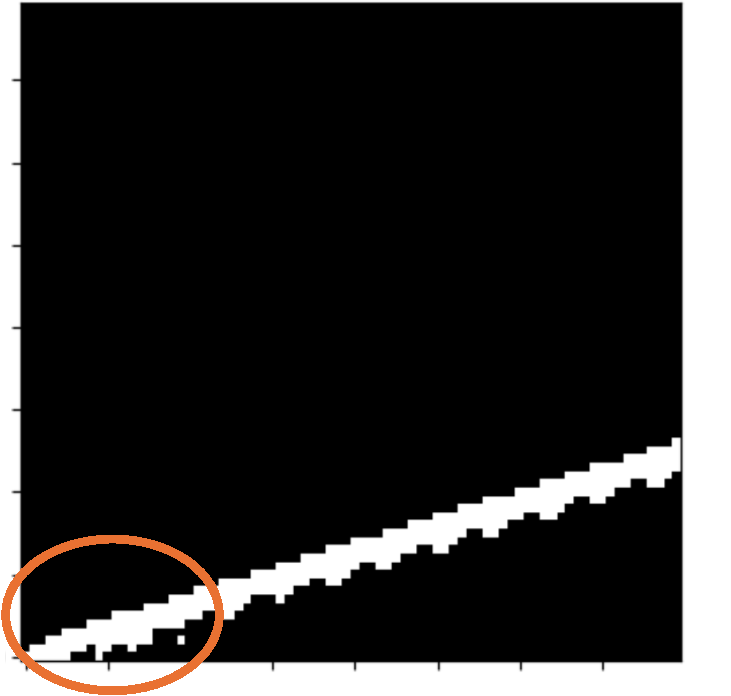
\includegraphics[width=\linewidth]{extracta.pdf}
    \caption{SC法の結果から速度発散を計算し圧縮性の顕著なcell(白cell)を特定[\ref{subsubsec:comp}節].}
  \end{subfigure}
  \hfill
  \begin{subfigure}[t]{0.23\textwidth}
    \centering
    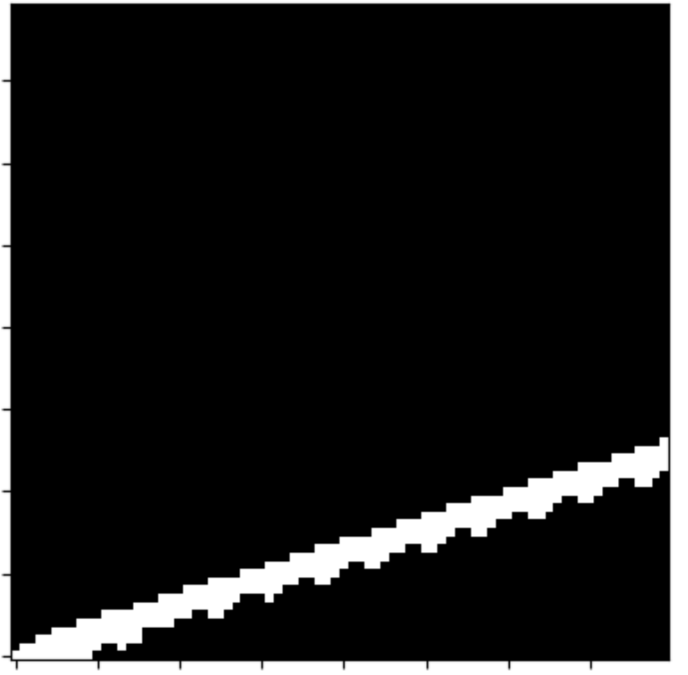
\includegraphics[width=\linewidth]{extractb.pdf}
    \caption{CCLでノイズを除去[\ref{subsubsec:CCL}節]. (a)の楕円内のノイズが除かれる.}
  \end{subfigure}
  % 下段
  \begin{subfigure}[t]{0.235\textwidth}
    \centering
    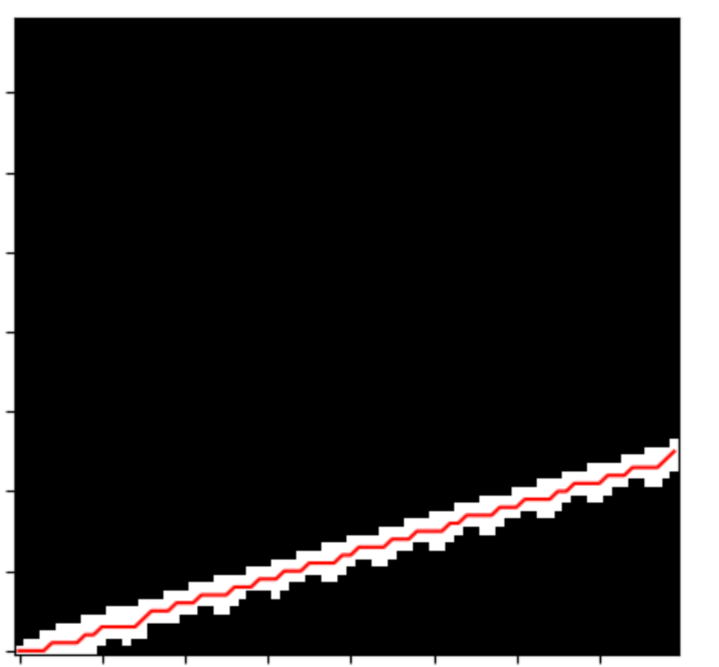
\includegraphics[width=\linewidth]{extractc.pdf}
    \caption{Skeleton化で主要骨格(赤線)を抽出[\ref{subsubsec:skeleton}節].}
  \end{subfigure}
  \hfill
  \begin{subfigure}[t]{0.23\textwidth}
    \centering
    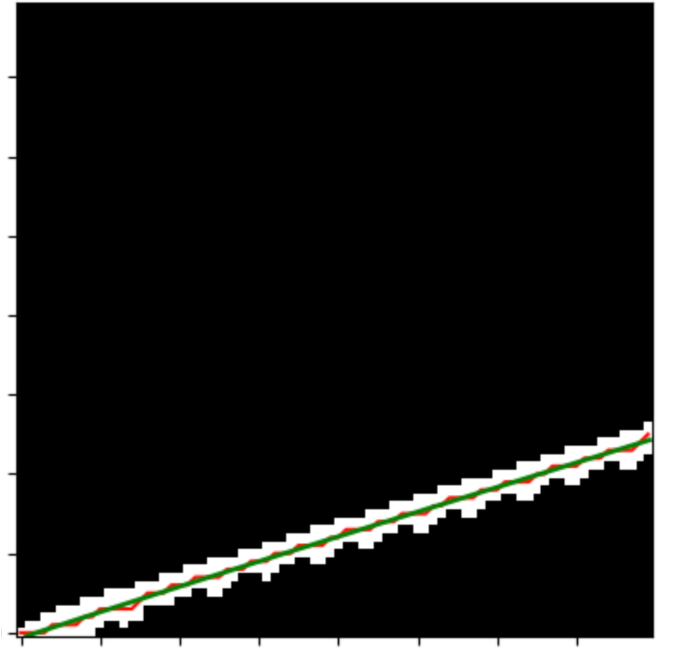
\includegraphics[width=\linewidth]{extractd.pdf}
    \caption{Spline近似で滑らかな衝撃波面(緑線)を得る[\ref{subsubsec:spline}節].}
  \end{subfigure}

  \caption{SC法の結果から不連続領域を抽出し初期衝撃波面を推定する手順[\ref{subsec:discon}節].}
  \label{fig:extract}
\end{figure}
\subsection{Shock-Fitting法}
\mbox{}\\[-3.0ex]

\subsubsection{Blanked cells, Adjoining Boundary cells, Surrogate Boundary cellsのラベリング} \label{subsubsec:boundary}
\mbox{}\\[1.0ex]
背景の直交格子のcellで, shock-pointsを繋いだshock-edge(衝撃波面に相当)に横切られるcellを,
Blanked cellsと呼ぶ. 
Blanked cellsに少なくとも一辺を接しているcellをAdjoining Boundary cellsと定義する.
さらに, Adjoining Boundary cellsと少なくとも一辺または一つの頂点を共有するcellを
Surrogate Boundary cellsと定義する.

ただし, 以下の条件を満たすように微修正を行う.
\begin{itemize}
  \item[・]  全てのAdjoining Boundary cellsは, 少なくとも一辺をSurrogate Boundary cellsと共有する.
  そうでないものは、Blanked cellsにする.
  \item[・]  全てのSurrogate Boundary cellsは、上下または左右からAdjoining Boundary cellsやGhost cellsに挟まれない.
  挟まれる場合, Adjoining Boundary cellsにする.
\end{itemize}
Figure.\ref{fig:grouping}は斜め衝撃波の衝撃波面の周囲で, 実際にラベリングを行った例である.

\vskip\baselineskip
\begin{figure}[H]
    \vspace*{-5mm}
    \begin{center}
        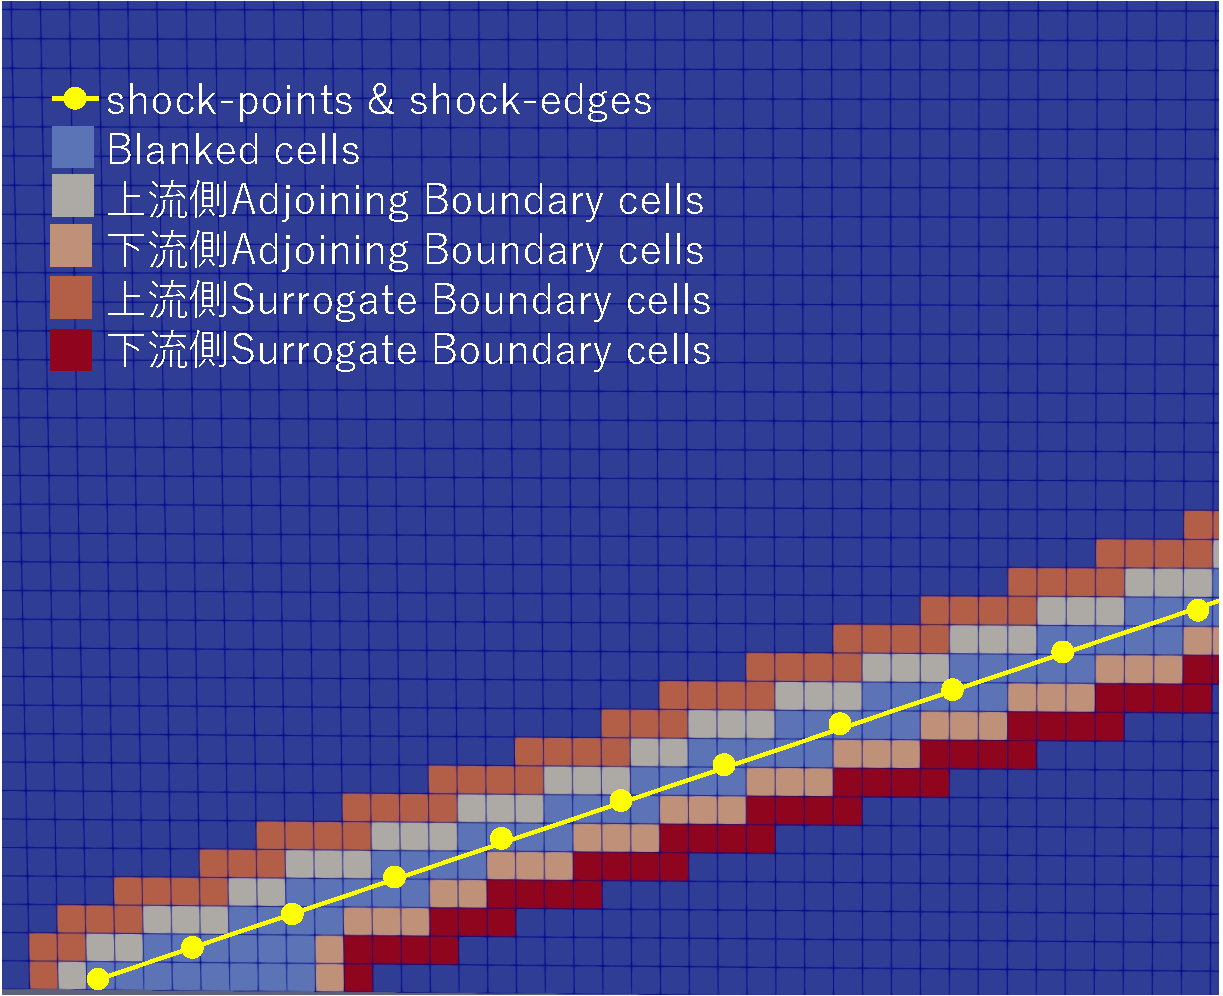
\includegraphics[width=0.45\textwidth]{grouping.pdf}
    \end{center}
    \caption{Shock-fitting法におけるcellのグルーピングの例.
    衝撃波面に横切られるcellをBlanked cells, その1層外側がAdjoining Boundary, さらに1層外側が
    Surrogate Boundary. さらに\ref{subsubsec:boundary}節の諸条件を満たすよう修正する.}
    \label{fig:grouping}
\end{figure}

%\ref{subsubsec:sc}節で衝撃波上流領域と下流領域でSC法を独立に実行する際, Adjoining Boundaryは境界条件を課すcellとして働く.
%Suroogate BoundaryからがFVMの対象になり, 計算領域の境界を表す.

\subsubsection{上流cell・下流cellの識別} \label{subsubsec:udflow}
\mbox{}\\[-1.0ex]

Adjoing Boundary cellsとSurrogate Boundary cellsが, それぞれ衝撃波の上流か下流どちらにあるかを判別する.
最初のタイムステップでは, shock-pointでの衝撃波法線と最近傍shock-pointからの相対位置ベクトルの内積を取り, 内積値の符号の正負によって2グループに分ける.
Figure.\ref{fig:updownjudge}では, 左上のcellは内積が正, 右下のcellは負であるので, この2つのcellは一方が衝撃波上流側, もう一方が下流側と判別できる.
その2グループのcellにおける圧力値を衝撃波面を跨いで比較し, 圧力が高い方を衝撃波下流側と判定する.

次回以降のステップでは, \ref{subsubsec:normal}節で衝撃波法線方向を衝撃波上流方向に限定しているため, 
内積値の符号のみで上流・下流の識別が可能である.

\vskip\baselineskip
\begin{figure}[H]
    \vspace*{-5mm}
    \begin{center}
        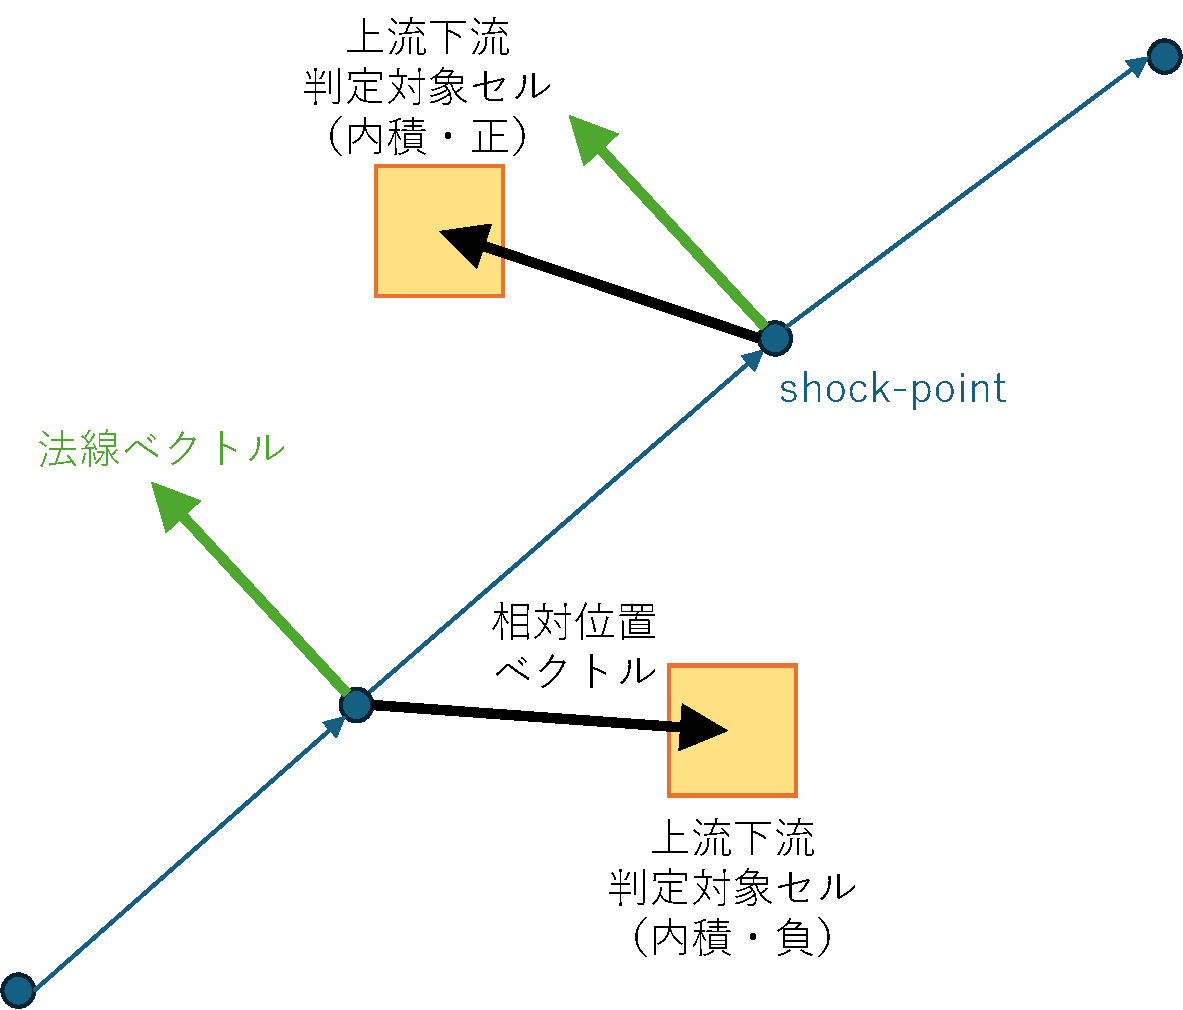
\includegraphics[width=0.45\textwidth]{updownjudge.pdf}
    \end{center}
    \caption{上流・下流判定対象cellに対し, 最近傍shock-pointからの相対位置ベクトル(黒)と衝撃波法線(緑)の内積を取る.
    左上のcellは内積が正, 右下のcellは負である.  一方が衝撃波上流側, もう一方が下流側と判別できるので, 圧力値を比較し高いほうが下流側である.}
    \label{fig:updownjudge}
\end{figure}

\subsubsection{外挿に不要なshock-pointsの除去} \label{subsubsec:remove}
\mbox{}\\[-1.0ex]

Shock-pointsの持つ上流値, 下流値は\ref{subsubsec:adjoining}節でAdjoinind Boundaryに値を
外挿する際に用いられる. そのため, どのAdjoing Boundary cellsからも近くなく, 外挿時に参照されないshock-pointsは全く不要であるので,
あらかじめ取り除く. この操作は最初のタイムステップのみ行う.

\subsubsection{SC法ソルバーによる計算領域でのCFDの実行} \label{subsubsec:sc}
\mbox{}\\[-1.0ex]
衝撃波上流領域と下流領域でSC法を独立に実行する. SC法で課した境界条件に加え, 衝撃波上流側Adjoining Boundaryと
下流側Adjoining Boundaryに境界条件を課す.
\begin{itemize}
  \item[・]  衝撃波上流側Adjoining Boundary:対象Adjoining Boundary cellの縦横斜め8近傍でSurrogate Boundary cellsを探索する. 
            そのcellでの速度方向が最も対象Adjoining Boundary cellに向いているSurrogate Boundary cellの値を, 対象Adjoining Boundary cellに複製する. 流出・流入境界条件(0次外挿)に相当する.
  \item[・]  衝撃波下流側Adjoining Boundary:もともとcellの持っている値を保持する. この値は各タイムステップの
            \ref{subsubsec:adjoining}節のプロセスで更新される.
\end{itemize}

\subsubsection{Surrogate Boundary cellsからshock-pointsへの値の外挿} \label{subsubsec:extrapolate}
\mbox{}\\[-1.0ex]

時間更新されたSurrogate Boundary cellsで基本変数の勾配をGreen-Gauss法により計算する$^{(\ref{ref:SF})}$.
この結果を用いて, 各shock-pointに対し, 近傍のSurrogate Boundary cellから基本変数の値を1次外挿する$^{(\ref{ref:SF})}$.
各shock-pointは上流値と下流値の二つの値を持つが,
上流側のSurrogate Boundaryは超音速流出境界で上流方向に特性曲線が伝播しないため, 
すべての基本変数を外挿する.

一方で, 下流値については遅い音響波(slow acoustic wave)に対応するリーマン変数のみを外挿する.
衝撃波下流領域から特性曲線に乗って衝撃波面に伝わる情報は, このひとつのみだからである.
下流側から外挿するリーマン変数は次式で与えられる.

\begin{equation}
    R_d^{t+\Delta t} = \tilde{a}_d^{t+\Delta t} + \frac{\gamma - 1}{2}\tilde{\mathbf{u}}_d^{t+\Delta t} \cdot \mathbf{n}
    \label{eq:Riemann_down}
\end{equation}

ここで,$\tilde{a}_d^{t+\Delta t}$ および $\tilde{\mathbf{u}}_d^{t+\Delta t}$ は
下流側Surrogate Boundaryから外挿された仮の音速および速度ベクトルであり, 
$\mathbf{n}$ は衝撃波法線ベクトルである.
CFD計算における風上差分の性質により,
式(\ref{eq:Riemann_down})の左辺に相当するリーマン変数 $R_d^{t+\Delta t}$ は正しく時間発展している一方で,
右辺の外挿量(チルダ付き)は近似値に過ぎない.
これらの量は\ref{subsubsec:rankine}節でR-H条件を課すことにより修正される.

\subsubsection{衝撃波法線ベクトルの計算} \label{subsubsec:normal}
\mbox{}\\[-1.0ex]

各shock-pointにおいて, 衝撃波法線ベクトルを計算する. このとき, 周辺のshock-pointsが"影響範囲$^{(\ref{ref:effdomain})}$"に含まれるかを判断し,
風上2点分のshock-pointsの座標, または風上風下両側2点分の座標を用いて計算する$^{(\ref{ref:SF})}$.
衝撃波法線ベクトルは衝撃波上流方向を向くものを採用する.

\subsubsection{Shock-pointsでのRankine-Hugoniot条件の適用} \label{subsubsec:rankine}
\mbox{}\\[-1.0ex]

各shock-pointsにおいてR-H条件を適用する.
求解対象となる変数は, 衝撃波下流側の密度$\rho_d$, 衝撃波法線方向速度$u_n^d$, 接線方向速度$u_\tau^d$, 
圧力$p_d$, およびshock-point速度$w_s$の計5変数である.これらに対して, 以下の5つの式が構成される.

\begin{equation}\label{eq:R-H}
\begin{aligned}
 \rho_d (u_n^d - w_s) &= \rho_u (u_n^u - w_s) \\
 \rho_d (u_n^d - w_s)^2 + p_d &= \rho_u (u_n^u - w_s)^2 + p_u \\
 \frac{\gamma}{\gamma - 1} \frac{p_d}{\rho_d} + \frac{1}{2}(u_n^d - w_s)^2 &= \frac{\gamma}{\gamma - 1} \frac{p_u}{\rho_u} + \frac{1}{2}(u_n^u - w_s)^2\\
 u_\tau^d &= u_\tau^u\\
 a_d + \frac{\gamma - 1}{2} u_n^d &= R_d 
\end{aligned}
\end{equation}
\vskip\baselineskip
上付き添字$u$と$d$はそれぞれ衝撃波の上流および下流側を意味し, $a_d$は下流側音速, 
$R_d$は下流側のリーマン変数である. なお, 全ての物理量について上付添字$t+\Delta t$を省略している.

\subsubsection{時間積分によるShock Nodesの進行} \label{subsubsec:prop}
\mbox{}\\[-1.0ex]

\ref{subsubsec:rankine}節で得たshock-point速度$w_s$を使用し, shock-pointsの位置を更新する.
非定常問題への対応や高次精度の要求を満たすため, 高次の陽的多段法である
Adams-Bashforth法を用いる.

\subsubsection{Shock-pointsから下流Adjoining Boundary, Blanked cellsへの値の外挿} \label{subsubsec:adjoining}
\mbox{}\\[-1.0ex]

各shock-pointで, 基本変数の勾配を計算する.
近傍のshock-point, 下流Surrogate Boundary cellの基本変数値とその相対位置から, 
基本変数場をshock-point周りに線形近似する$^{(\ref{ref:SF})}$.
この際, 使用するshock-pointは\ref{subsubsec:normal}節で考えた"影響範囲"をもとに選択する.
求めた基本変数場から, Blanked cells, 下流Adjoing Bondary cellsの位置での各基本変数値が得られる.
Blanked cellsは, shock-pointsの移動によりCFD対象cellに変化する可能性があるため,
毎時間ステップごとに値を更新する.

以上のプロセスにより, 全てのcellの基本変数値, shock-pointsの持つ上流・下流値とその位置が時間更新される.

\section{結果}
\subsection{1次元非定常垂直衝撃波}\label{subsec:1D}
\mbox{}\\[-3.0ex]

最も単純な1次元非定常垂直衝撃波を扱い, SF法の基本的な挙動と精度, 非定常問題への追従性を確認する.
Figure.\ref{fig:1Dsituation}に計算領域・設定の概略を示す.
衝撃波は最初に$x=0.5$に存在し, 速度$w=-0.2$で移動する.
上流・下流の基本変数はこの条件を成立させるよう, あらかじめR-H条件を解いて与える.
SC法の計算では, x軸方向に50cellの直交格子を用いる.
1タイムステップの時間幅は, CFL条件を満たす固定値として設定し, $\Delta t = 0.001$とする.
\begin{figure}[H]
    \vspace*{-5mm}
    \begin{center}
        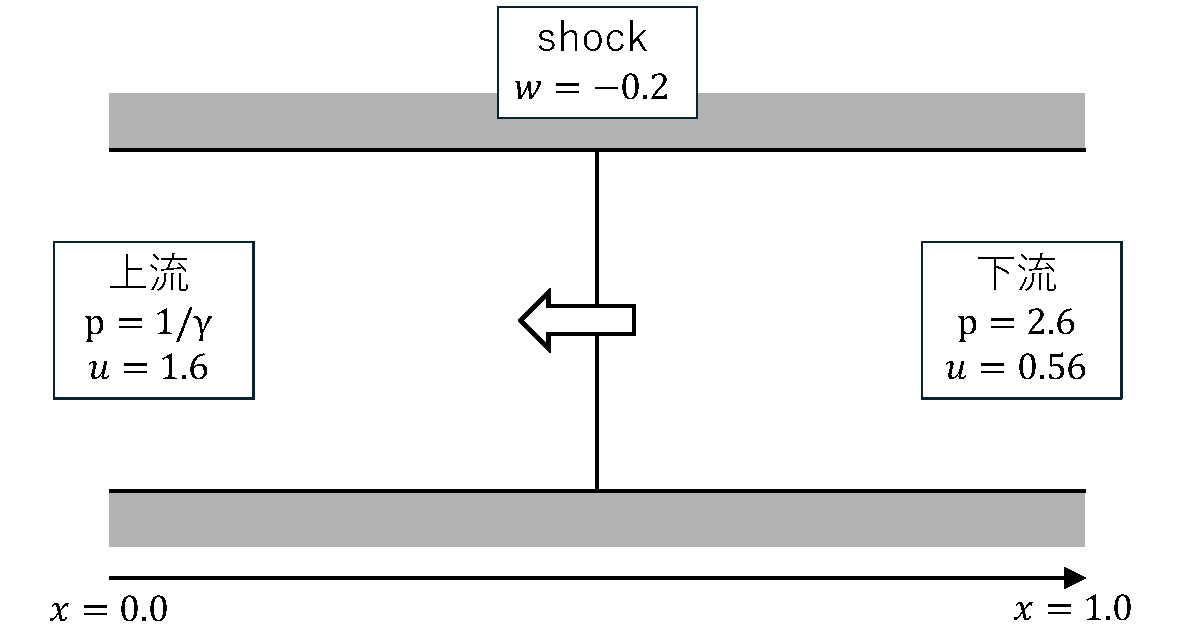
\includegraphics[width=0.4\textwidth]{1Dsituation.pdf}
    \end{center}
    \caption{1次元非定常垂直衝撃波の計算領域・設定の概略.
    衝撃波は最初に$x=0.5$に存在し, 速度$w=-0.2$で移動する.}
    \label{fig:1Dsituation}
\end{figure}
SF法による計算の結果, 衝撃波速さは常に0.20000000298023216という値となった.
理論解との差は, \ref{subsubsec:rankine}節でのニュートンラプソン法実行時の収束閾値が由来であった. 
残差は倍精度の機械イプシロンまで収束していた. また, 流れ場は常に理論解と一致した.

Figure.\ref{fig:1Dscsf}上図は, SC法の結果(青)とSF法の結果(赤)を密度について比較している(1500step, t=1.5).
SC法では, 衝撃波が人工粘性により平滑化され, 衝撃波位置が不明確である.
また, SC法の結果は衝撃波上流側では理論解と完全に一致するが, 衝撃波下流域では
数値振動が発生し理論解と差を生じる.
Figure.\ref{fig:1Dscsf}下図は, 衝撃波下流域の密度分布について, SC法の結果と理論解との差を示している.
衝撃波前後の密度変化の0.1\%程度の振幅の数値的減衰振動が確認できる.
\vskip\baselineskip
\begin{figure}[H]
    \vspace*{-5mm}
    \begin{center}
        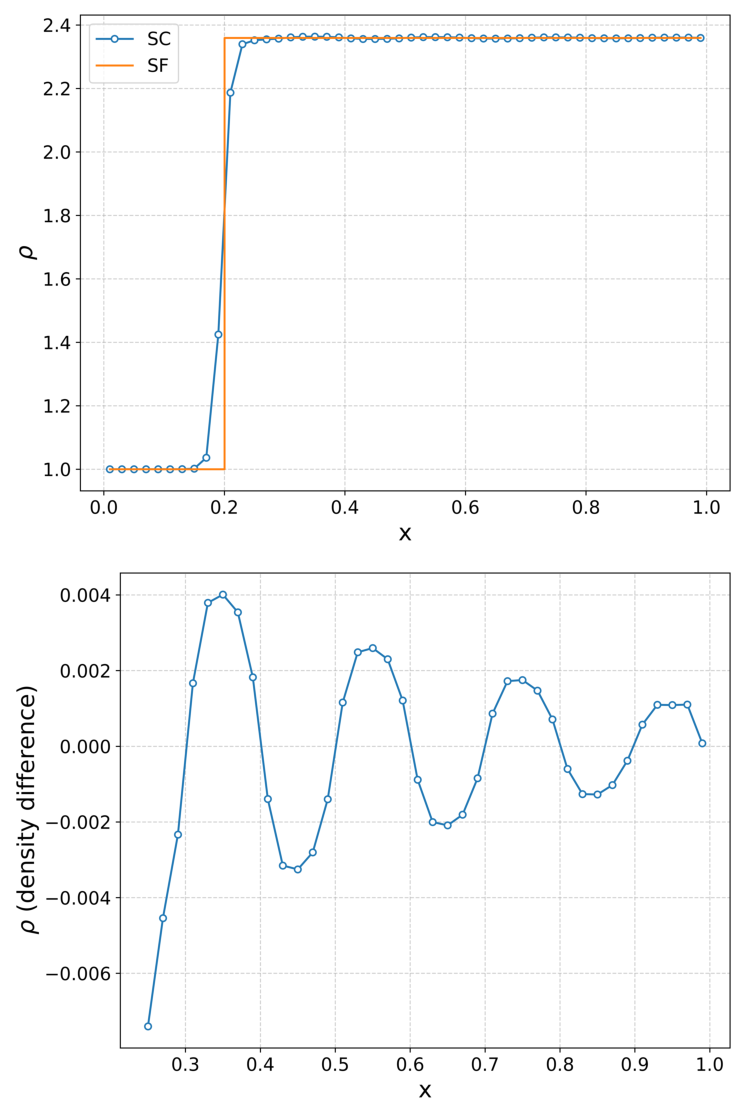
\includegraphics[width=0.45\textwidth]{1Dscsf.pdf}
    \end{center}
    \caption{上:1次元非定常垂直衝撃波のSC法の結果(青)とSF法の結果(赤)を密度について比較(1500step, t=1.5).\\
    下:衝撃波下流域密度分布の, SC法の結果と理論解との差.
    }
    \label{fig:1Dscsf}
\end{figure}

\subsection{2次元定常斜め衝撃波}\label{subsec:2Ddiag}
\mbox{}\\[-3.0ex]

2次元定常斜め衝撃波を扱い, 衝撃波面が背景格子に沿わない2次元流れでのSF法の挙動と精度を確認する.
Figure.\ref{fig:2Ddiagsituation}に計算領域・設定の概略を示す.
計算領域左端から, マッハ数$M_\infty=2.5$, 角度$\theta=15^\circ$の均一流を流入する.
下端は滑り壁条件である. SC法で1000step計算した後, \ref{subsec:discon}節のプロセスで衝撃波面を抽出し, SC法, SF法でそれぞれ保存量の残差が$10^{-14}$を下回るまで
計算を継続する.
\vskip\baselineskip
\begin{figure}[H]
    \vspace*{-5mm}
    \begin{center}
        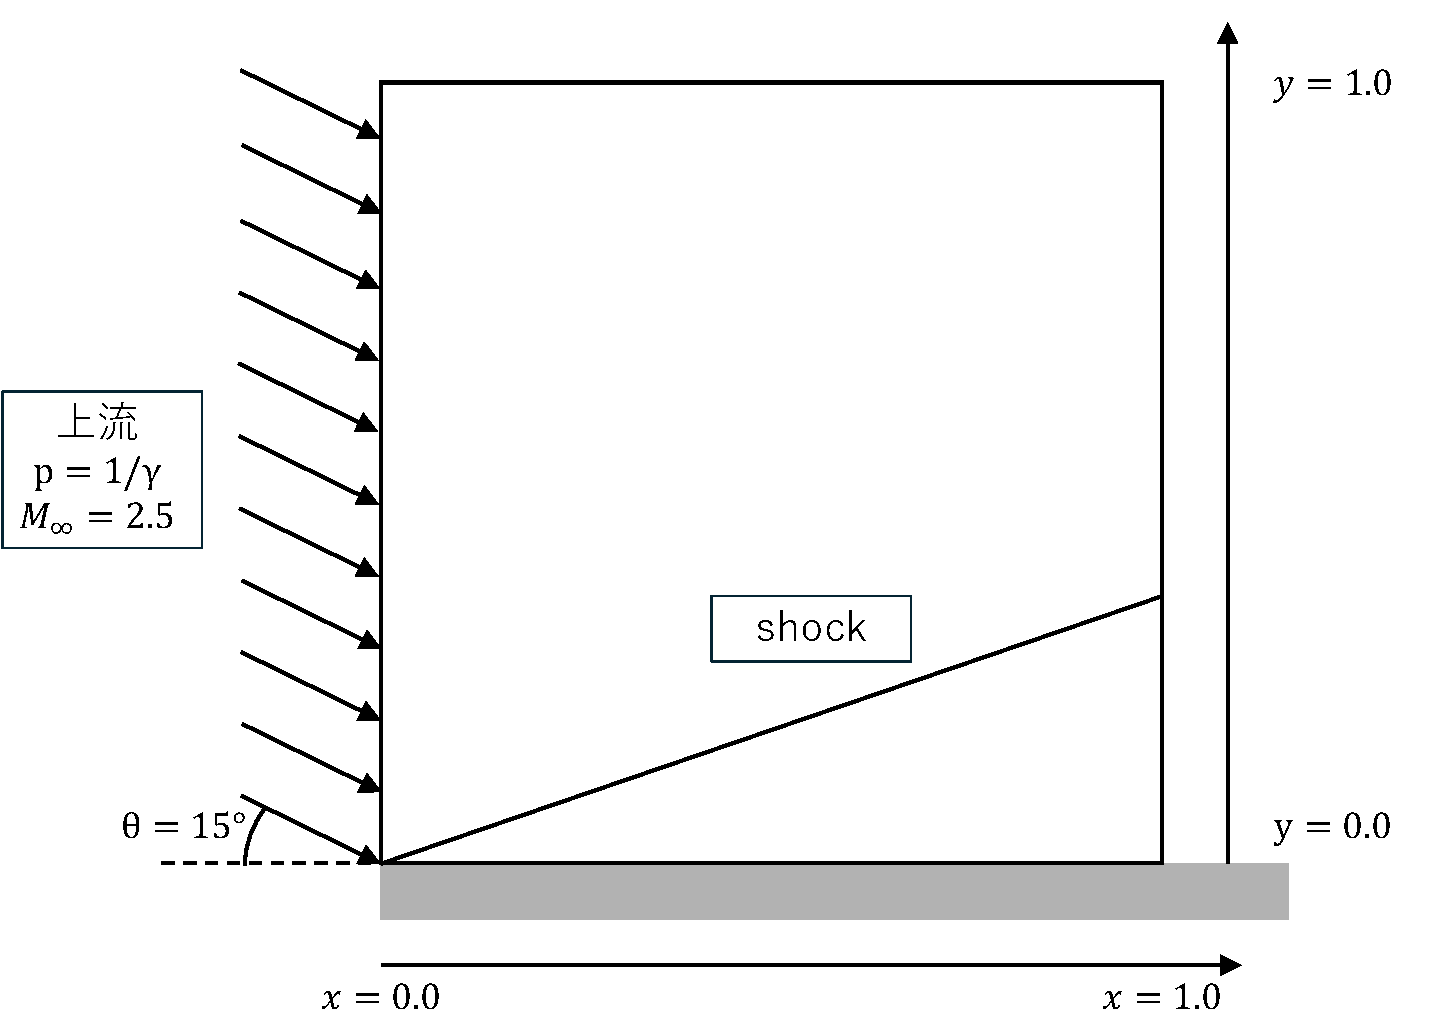
\includegraphics[width=0.45\textwidth]{2Ddiagsituation.pdf}
    \end{center}
    \caption{2次元定常斜め衝撃波の計算領域・設定の概略.
    計算領域左端から, マッハ数$M_\infty=2.5$, 角度$\theta=15^\circ$の均一流を流入する.
    下端は滑り壁条件.}
    \label{fig:2Ddiagsituation}
\end{figure}

SC法, SF法での計算結果を解析解と比較する.
衝撃波の不連続が存在する領域は, SC法では正確に表現できないことが明らかであるため,
圧縮性が顕著なcell(\ref{subsubsec:comp}節)を除いた計算領域で比較を行う.
Figure.\ref{fig:2Ddiagcomp}上は, SC法の密度分布と解析解の差を示す.
衝撃波後流域に数値的減衰振動が発生していることが確認できる.
誤差は, 衝撃波前後の密度変化の約10\%のオーダーに達している.
衝撃波面から離れるに従い, 誤差が減少することもわかる.
一方, Fig.\ref{fig:2Ddiagcomp}下は, SF法の密度分布と解析解の差を示す.
誤差は衝撃波前後の密度変化の$10^{-10}$のオーダーに抑えられており, 数値振動は見られない.

\vskip\baselineskip
\begin{figure}[H]
    \vspace*{-5mm}
    \begin{center}
        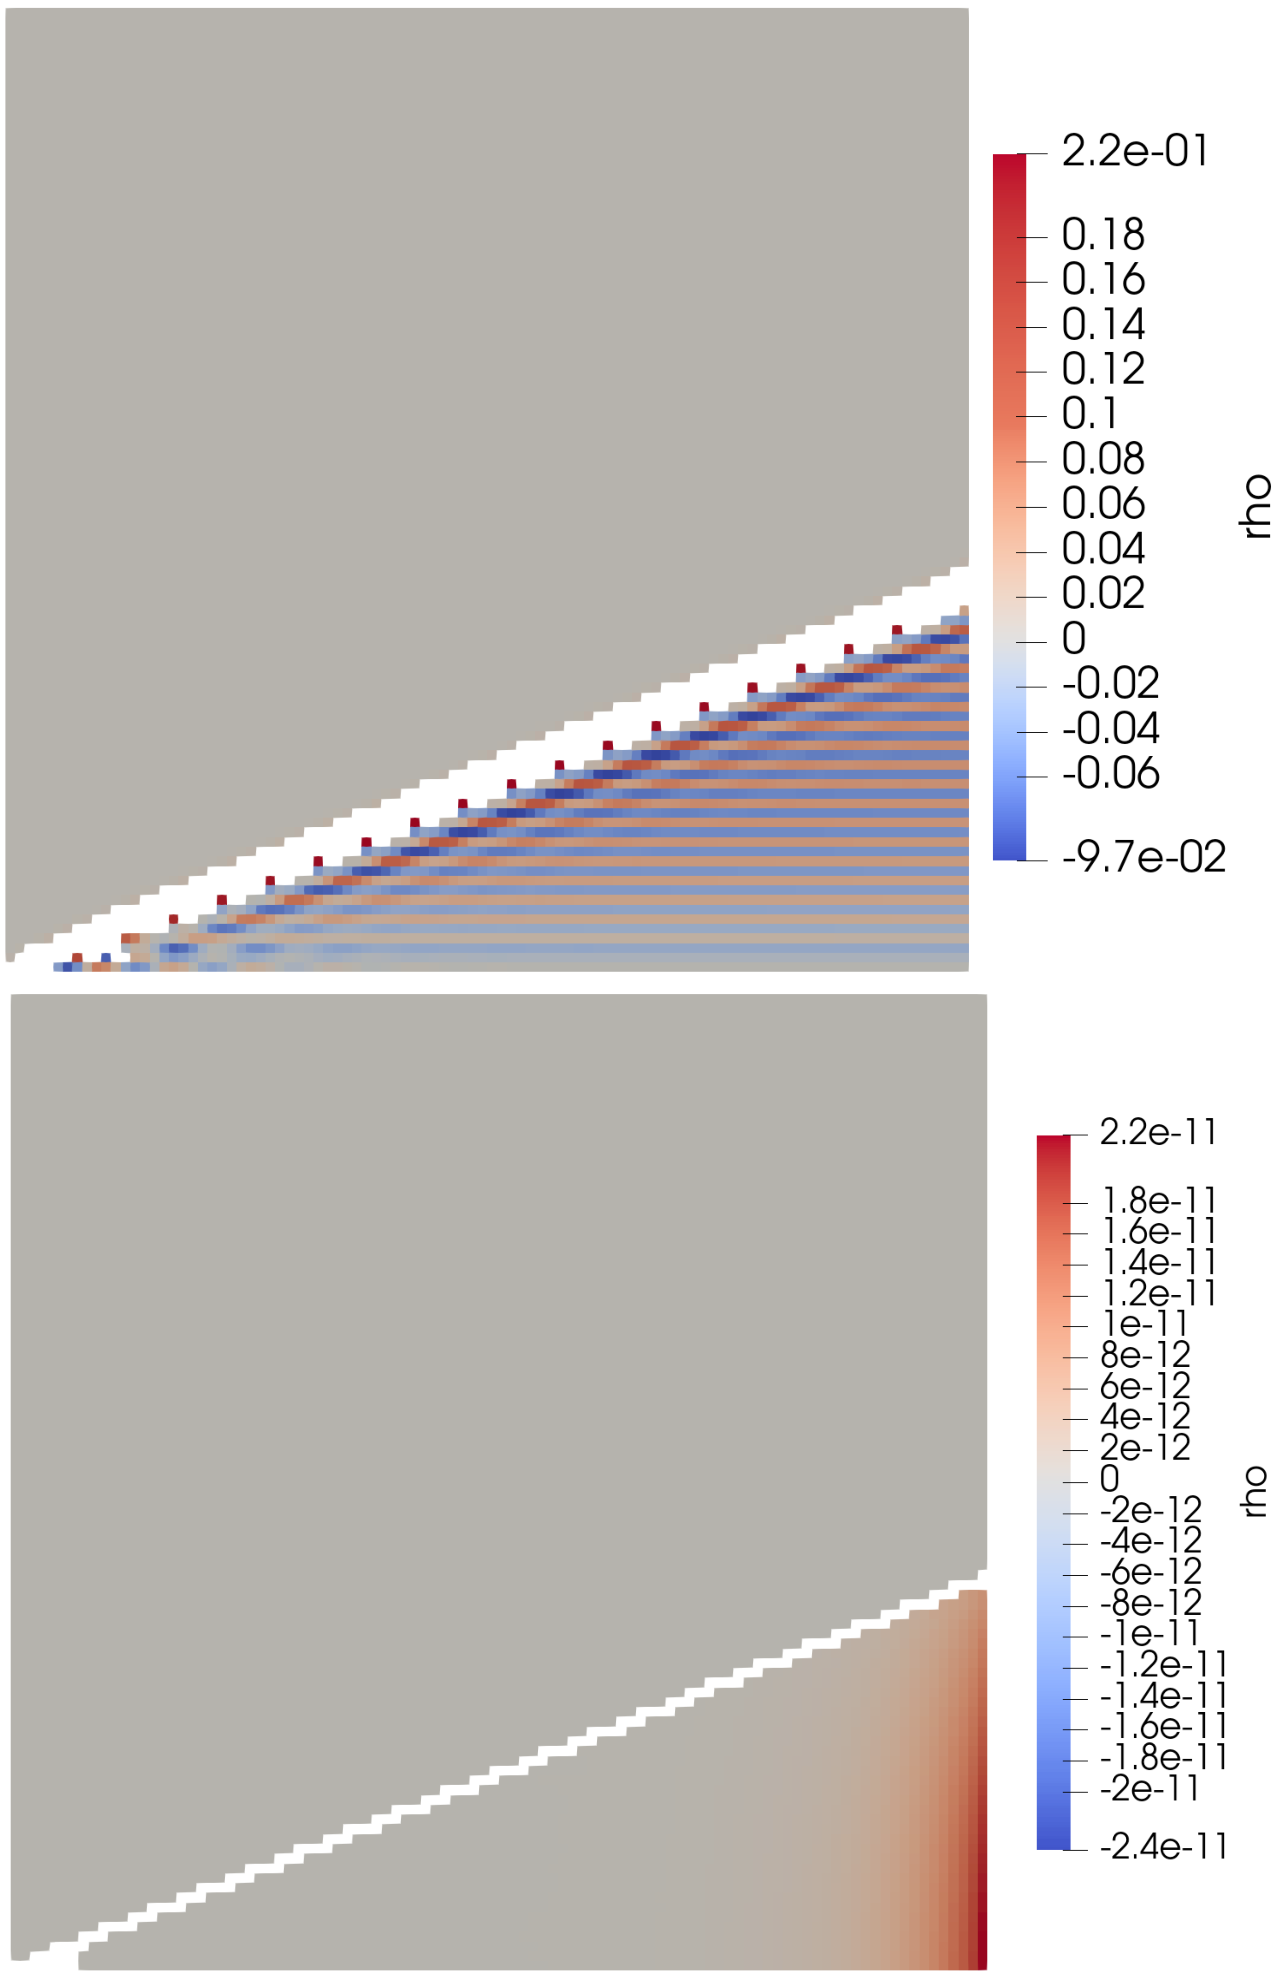
\includegraphics[width=0.45\textwidth]{2Ddiagcomp.pdf}
    \end{center}
    \caption{2次元定常斜め衝撃波のSC法, SF法計算結果(密度分布)の解析解との差分. 空白cellは不連続領域. \\
    上:SC法と解析解の差分.衝撃波後流域に数値振動が発生している. \\
    下:SF法と解析解の差分. 数値振動は見られない.}
    \label{fig:2Ddiagcomp}
\end{figure}

\subsection{2次元定常角柱離脱衝撃波}\label{subsec:2Dsq}
\mbox{}\\[-3.0ex]

2次元定常角柱離脱衝撃波を解析し, 流れ場の基本変数分布に非一様性があり, 衝撃波面が曲率を持つ場合のSF法の挙動を確認する.
Figure.\ref{fig:2Dcolumnsitu}に計算領域・設定の概略を示す.
計算領域左端から, マッハ数$M_\infty=4.0$の一様流を流入する.
角柱表面は滑り壁条件を課す. 
\vskip\baselineskip
\begin{figure}[H]
    \vspace*{-5mm}
    \begin{center}
        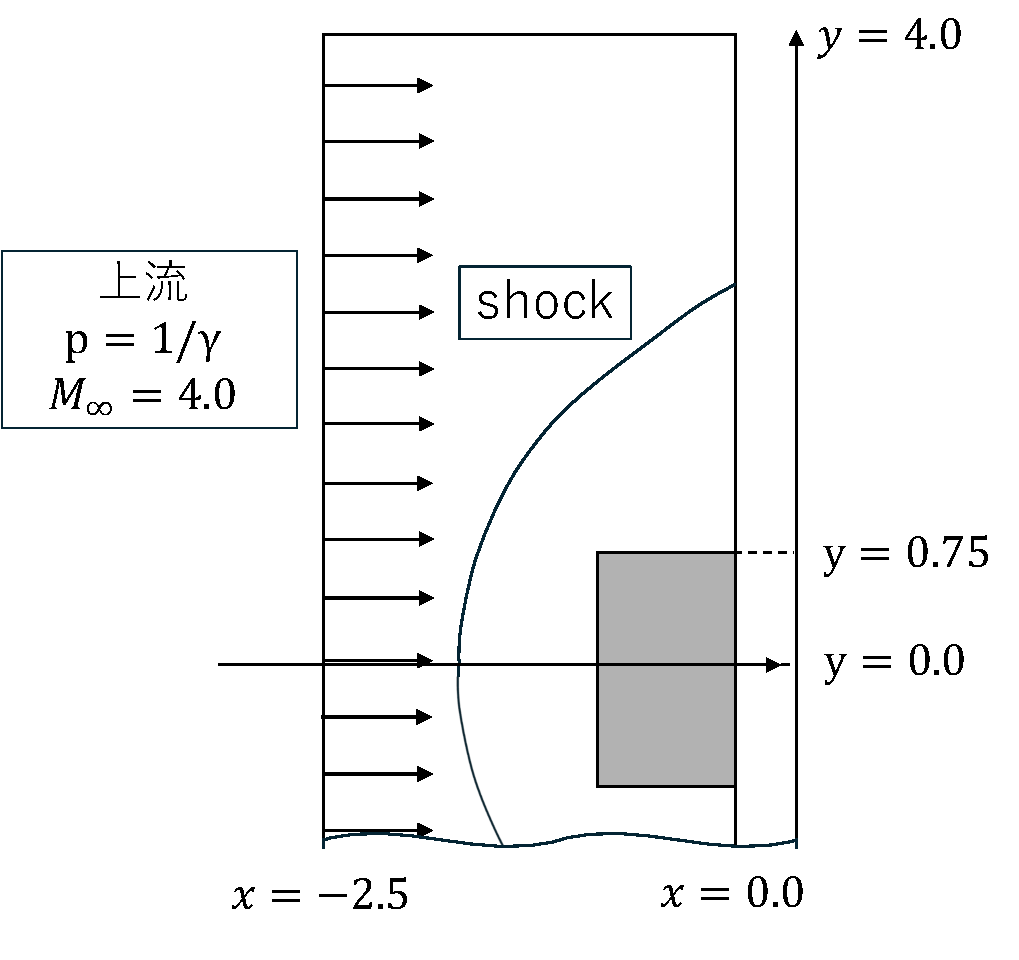
\includegraphics[width=0.45\textwidth]{2Dcolumnsitu.pdf}
    \end{center}
    \caption{2次元定常角柱離脱衝撃波の計算領域・設定の概略.
    計算領域左端から, マッハ数$M_\infty=4.0$の一様流を流入する.
    角柱表面は課す.}
    \label{fig:2Dcolumnsitu}
\end{figure}
淀み点の基本変数を用いて格子収束性を確認, 理論値, SCと比較などする予定

\subsection{2次元定常円柱離脱衝撃波}\label{subsec:2Dcirc}
\mbox{}\\[-3.0ex]

未定。IB法とも併用できるよ, くらいになるかも.

\clearpage
\section{結論}

\section*{参考文献}

\begin{enumerate}
    \item Ciallella, M., Ricchiuto, M., Paciorri, R. and Bonfiglioli, A., ``Extrapolated Discontinuity Tracking for complex 2D shock interactions,''
     Computers \& Fluids, Vol. 391 (2022), pp. 114543.
\label{ref:eDIT}
    \item Assonitis, A., Ciallella, M., Paciorri, R., Ricchiuto, M. and Bonfiglioli, A., ``A new shock-fitting technique for 2-D structured grids,''
     AIAA SCITECH 2022 Forum, Paper 2022-2008 (2022).
\label{ref:SESF}
    \item Assonitis, A., Paciorri, R., Ciallella, M., Ricchiuto, M. and Bonfiglioli, A., ``Extrapolated Shock Fitting for Two-Dimensional Flows on Structured Grids,''
     AIAA J., Vol. 60, No. 11 (2022), pp. 6301-6312.
\label{ref:SF}
    \item Yoshiharu, T., Motoshi, H. and Taro, I., ``Near-Wall Modification of Spalart–Allmaras Turbulence Model for Immersed Boundary Method,''
     AIAA J., Vol. 55, No. 9 (2017), pp. 3027-3039.
\label{ref:IBM}
    \item De Zeeuw, D. and Powell, K. G., ``Euler Calculations of Axisymmetric Under-Expanded Jets by an Adaptive-Refinement Method,''
     30th Aerospace Sciences Meeting \& Exhibit, Paper 92-0321 (1992), pp. 1-13. 
\label{ref:AMR}
    \item Zhang, T. Y. and Suen, C. Y., ``A fast parallel algorithm for thinning digital patterns,''  
     Communications of the ACM, Vol. 27, No. 3 (1984), pp. 236-239.
\label{ref:skelton}
    \item Paciorri, R. and Bonfiglioli, A., ``Accurate detection of shock waves and shock interactions in two-dimensional shock-capturing solutions,''
     Journal of Computational Physics, Vol. 406 (2020), pp. 109196.
\label{ref:intera}
     \item Paciorri, R. and Bonfiglioli, A., ``A shock-fitting technique for 2D unstructured grids,''
      Computers \& Fluids, Vol. 38 (2009), pp. 715-726.
\label{ref:effdomain}
    \end{enumerate}

\end{document}
